\documentclass[11pt]{article}

\usepackage[a4paper,margin=0.92in]{geometry}
\usepackage[T1]{fontenc}
\usepackage[utf8]{inputenc}
\usepackage{lmodern}
\usepackage{microtype}
\usepackage{amsmath,amssymb,amsthm,mathtools}
\usepackage{booktabs,array}
\usepackage{graphicx}
\usepackage{enumitem}
\usepackage{xcolor}
\usepackage[hidelinks]{hyperref}

\graphicspath{{../figures/}}

\hypersetup{
  pdftitle={Completed Pandrosion Prime Atlases and Phase Destruction},
  pdfauthor={Ivan Besevic},
  pdfsubject={Pandrosion prime atlas, completed zeta, phase velocity, Riemann zeros},
  pdfkeywords={Pandrosion, Riemann zeta, completed zeta, Riemann-Siegel theta, Euler product, phase}
}

\newtheorem{definition}{Definition}[section]
\newtheorem{proposition}[definition]{Proposition}
\newtheorem{theorem}[definition]{Theorem}
\newtheorem{conjecture}[definition]{Conjecture}
\newtheorem{remark}[definition]{Remark}

\newcommand{\C}{\mathbb C}
\newcommand{\R}{\mathbb R}
\newcommand{\Pset}{\mathcal P}
\newcommand{\X}{\mathcal X}
\newcommand{\Z}{\mathcal Z}
\newcommand{\dd}{\,\mathrm d}
\DeclareMathOperator{\Ree}{Re}
\DeclareMathOperator{\Imm}{Im}

\title{Completed Pandrosion Prime Atlases and Phase Destruction\\[3pt]
\large The archimedean chart, phase velocity, and zero candidates}
\author{Ivan Besevic\\Independent Mathematical Research}
\date{May 2026}

\begin{document}
\maketitle

\begin{abstract}
Paper 025 introduced the prime Pandrosion atlas: each Euler factor is an
infinite geometric cell
\[
        (1-\ell^{-s})^{-1}
        =
        1+\ell^{-s}+\ell^{-2s}+\cdots,
\]
and the critical line \(\Re(s)=1/2\) is the equilibrium locus between the
direct chart \(\ell^{-s}\) and the reciprocal chart \(\ell^{-(1-s)}\).
The present paper adds the missing archimedean chart.  The completed zeta
factor
\[
        C(s)=\frac12 s(s-1)\pi^{-s/2}\Gamma(s/2)
\]
is treated as the infinite-place Pandrosion chart, while finite Euler cells
\[
        E_{\ell,N}(s)=1+\ell^{-s}+\cdots+\ell^{-(N-1)s}
\]
form the prime charts.  The completed finite atlas is
\[
        \X_{\Pset,N}(s)=C(s)\prod_{\ell\in\Pset}E_{\ell,N}(s).
\]

The main theorem is a phase-velocity identity.  Along any vertical line
\(s=\sigma+it\), away from zeros and poles,
\[
        \frac{\dd}{\dd t}\arg \X_{\Pset,N}(\sigma+it)
        =
        \Ree\left[
        \frac{C'}{C}(s)+
        \sum_{\ell\in\Pset}\frac{E'_{\ell,N}}{E_{\ell,N}}(s)
        \right].
\]
On the critical line, the archimedean part is the Riemann--Siegel theta
velocity
\[
        \vartheta'(t)
        =
        \frac12\Ree\,\psi\!\left(\frac14+\frac{it}{2}\right)
        -\frac12\log\pi.
\]
Thus the completed Pandrosion atlas separates the zero problem into two
explicit pieces: archimedean phase drift and prime-cell phase interference.
We then formulate the phase-destruction conjecture: nontrivial zeros of
\(\xi(s)\) should arise as limiting points where the balanced completed atlas
has simultaneous phase alignment and amplitude collapse.  This is not a proof
of the Riemann hypothesis; it is a concrete Pandrosion phase calculus extending
the chart-equilibrium theorem of Paper 025.
\end{abstract}

\paragraph{One-sentence summary.}
Paper 025 finds the critical line from direct/reciprocal chart balance; Paper
026 adds the gamma chart and studies the phase velocity whose destructive
alignment should produce zeta zeros.

\paragraph{Status.}
The finite phase-velocity identities are proved.  The convergence of
finite-atlas phase-destruction events to nontrivial zeros is stated as a
conjecture and a numerical research program.

\tableofcontents

\section{What 026 adds}

Paper 025 gave a geometric explanation for the critical line.  It did not
study zero locations.  The reason is structural: a line is selected by
logarithmic chart balance, but zeros require phase cancellation.  The zeta
function also has an archimedean factor.  Ignoring it loses the
Riemann--Siegel theta term, which controls the deterministic part of the phase
on the critical line.

The present paper therefore adds one object:
\[
        C(s)=\frac12s(s-1)\pi^{-s/2}\Gamma(s/2).
\]
The completed zeta function is
\[
        \xi(s)=C(s)\zeta(s),
        \qquad
        \xi(s)=\xi(1-s).
\]
In the Pandrosion atlas language, \(C(s)\) is the archimedean chart, while the
Euler factors are the prime charts.

\begin{figure}[htbp]
\centering
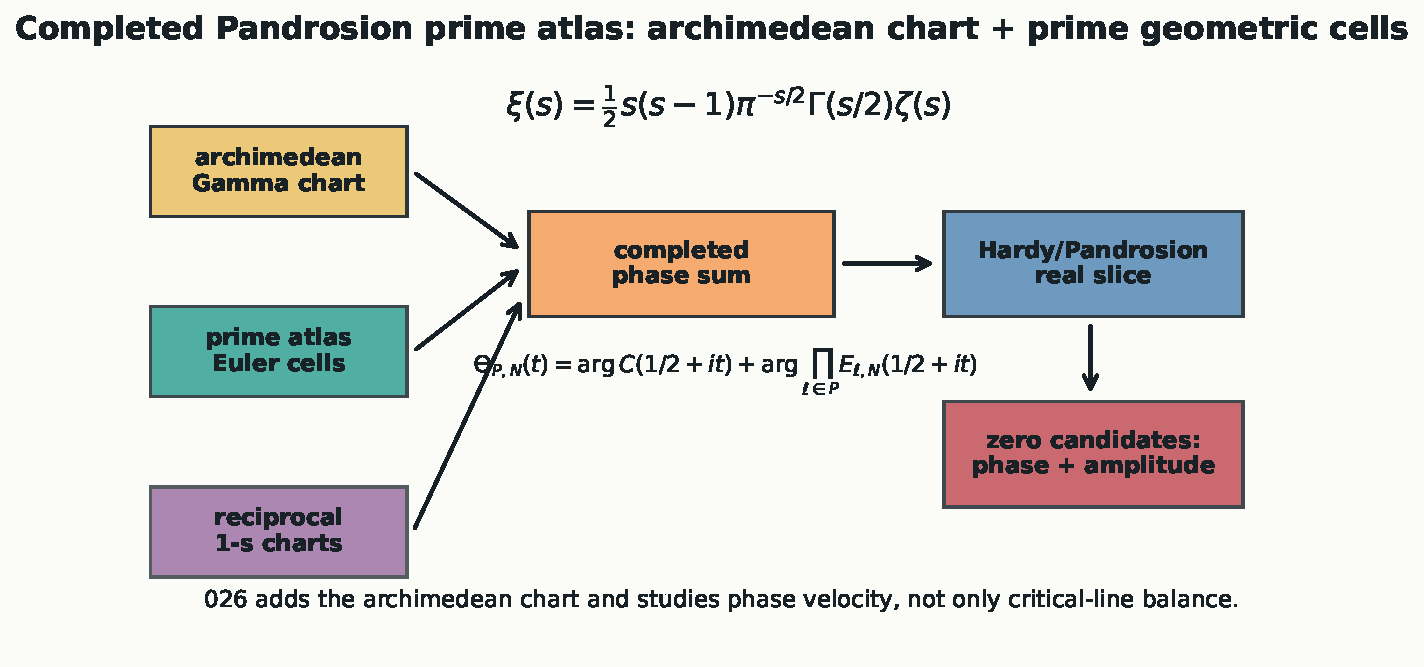
\includegraphics[width=0.98\linewidth]{026_completed_atlas_architecture.pdf}
\caption{Completed Pandrosion prime atlas.  The new ingredient beyond Paper
025 is the archimedean gamma chart \(C(s)\).  Zero candidates require both
phase alignment and amplitude collapse.}
\label{fig:completed-architecture}
\end{figure}

\section{Finite completed Pandrosion atlas}

Let \(\Pset\) be a finite set of primes and \(N\ge2\).  Define
\[
        E_{\ell,N}(s)
        =
        \sum_{r=0}^{N-1}\ell^{-rs}
        =
        \sum_{r=0}^{N-1}q_\ell(s)^r,
        \qquad
        q_\ell(s)=\ell^{-s}.
\]
The finite Euler-Pandrosion product is
\[
        \Z_{\Pset,N}(s)
        =
        \prod_{\ell\in\Pset}E_{\ell,N}(s),
\]
and the completed finite atlas is
\[
        \X_{\Pset,N}(s)
        =
        C(s)\Z_{\Pset,N}(s).
\]

\begin{remark}
For fixed \(\Pset,N\), this is not the completed zeta function.  It is a
finite model that exposes the two pieces of the phase: \(C(s)\) from the
infinite place and \(E_{\ell,N}\) from the prime geometric cells.
\end{remark}

\section{Phase velocity}

\begin{definition}[Vertical phase velocity]
Let \(F\) be holomorphic and nonzero near \(s=\sigma+it\).  Its vertical phase
velocity is
\[
        V_F(\sigma,t)
        =
        \frac{\dd}{\dd t}\arg F(\sigma+it).
\]
\end{definition}

\begin{lemma}[Basic phase derivative]
If \(F(s)\ne0\), then
\[
        V_F(\sigma,t)
        =
        \Ree\frac{F'}{F}(\sigma+it).
\]
\end{lemma}

\begin{proof}
Along the vertical path \(s(t)=\sigma+it\),
\[
        \frac{\dd}{\dd t}\log F(s(t))
        =
        i\,\frac{F'}{F}(s(t)).
\]
Taking imaginary parts gives
\[
        \frac{\dd}{\dd t}\arg F(s(t))
        =
        \Imm\left(i\,\frac{F'}{F}(s(t))\right)
        =
        \Ree\frac{F'}{F}(s(t)).
\]
\end{proof}

\begin{theorem}[Completed finite-atlas phase velocity]
Away from zeros and poles of \(\X_{\Pset,N}\),
\[
        \frac{\dd}{\dd t}\arg \X_{\Pset,N}(\sigma+it)
        =
        \Ree\left[
        \frac{C'}{C}(s)
        +
        \sum_{\ell\in\Pset}
        \frac{E'_{\ell,N}}{E_{\ell,N}}(s)
        \right]_{s=\sigma+it},
\]
where
\[
        \frac{C'}{C}(s)
        =
        \frac1s+\frac1{s-1}
        -\frac12\log\pi
        +\frac12\psi(s/2),
\]
and
\[
        E'_{\ell,N}(s)
        =
        -(\log\ell)
        \sum_{r=1}^{N-1}r\,\ell^{-rs}.
\]
\end{theorem}

\begin{proof}
The logarithmic derivative of a product is the sum of logarithmic
derivatives:
\[
        \frac{\X'_{\Pset,N}}{\X_{\Pset,N}}
        =
        \frac{C'}{C}
        +
        \sum_{\ell\in\Pset}
        \frac{E'_{\ell,N}}{E_{\ell,N}}.
\]
The displayed formula for \(C'/C\) follows by differentiating
\[
        \log C(s)=\log(1/2)+\log s+\log(s-1)-\frac{s}{2}\log\pi+\log\Gamma(s/2).
\]
The formula for \(E'_{\ell,N}\) follows from
\(\frac{\dd}{\dd s}\ell^{-rs}=-(r\log\ell)\ell^{-rs}\).
The basic phase derivative lemma completes the proof.
\end{proof}

\section{The archimedean chart and Riemann--Siegel theta}

On the critical line, write
\[
        s=\frac12+it.
\]
The Riemann--Siegel theta function is
\[
        \vartheta(t)
        =
        \Imm\log\Gamma\!\left(\frac14+\frac{it}{2}\right)
        -\frac{t}{2}\log\pi.
\]
It is the archimedean phase that makes
\[
        Z(t)=e^{i\vartheta(t)}\zeta(1/2+it)
\]
real for real \(t\).

\begin{proposition}[Archimedean phase velocity]
For real \(t\) away from branch choices,
\[
        \vartheta'(t)
        =
        \frac12\Ree\,\psi\!\left(\frac14+\frac{it}{2}\right)
        -\frac12\log\pi.
\]
Moreover, the phase velocity of \(C(1/2+it)\) differs from
\(\vartheta'(t)\) only by the constant branch contribution of
\(\frac12s(s-1)\), hence has the same derivative on intervals avoiding branch
cuts.
\end{proposition}

\begin{proof}
Differentiate the defining expression for \(\vartheta\):
\[
        \frac{\dd}{\dd t}
        \Imm\log\Gamma\!\left(\frac14+\frac{it}{2}\right)
        =
        \Imm\left(
        \frac{i}{2}\psi\!\left(\frac14+\frac{it}{2}\right)
        \right)
        =
        \frac12\Ree\,\psi\!\left(\frac14+\frac{it}{2}\right).
\]
The derivative of \(-t\log\pi/2\) is \(-\log\pi/2\).  On the critical line,
\(s(s-1)=-(t^2+1/4)\) is real negative, so its argument is constant between
branch jumps.
\end{proof}

\begin{figure}[htbp]
\centering
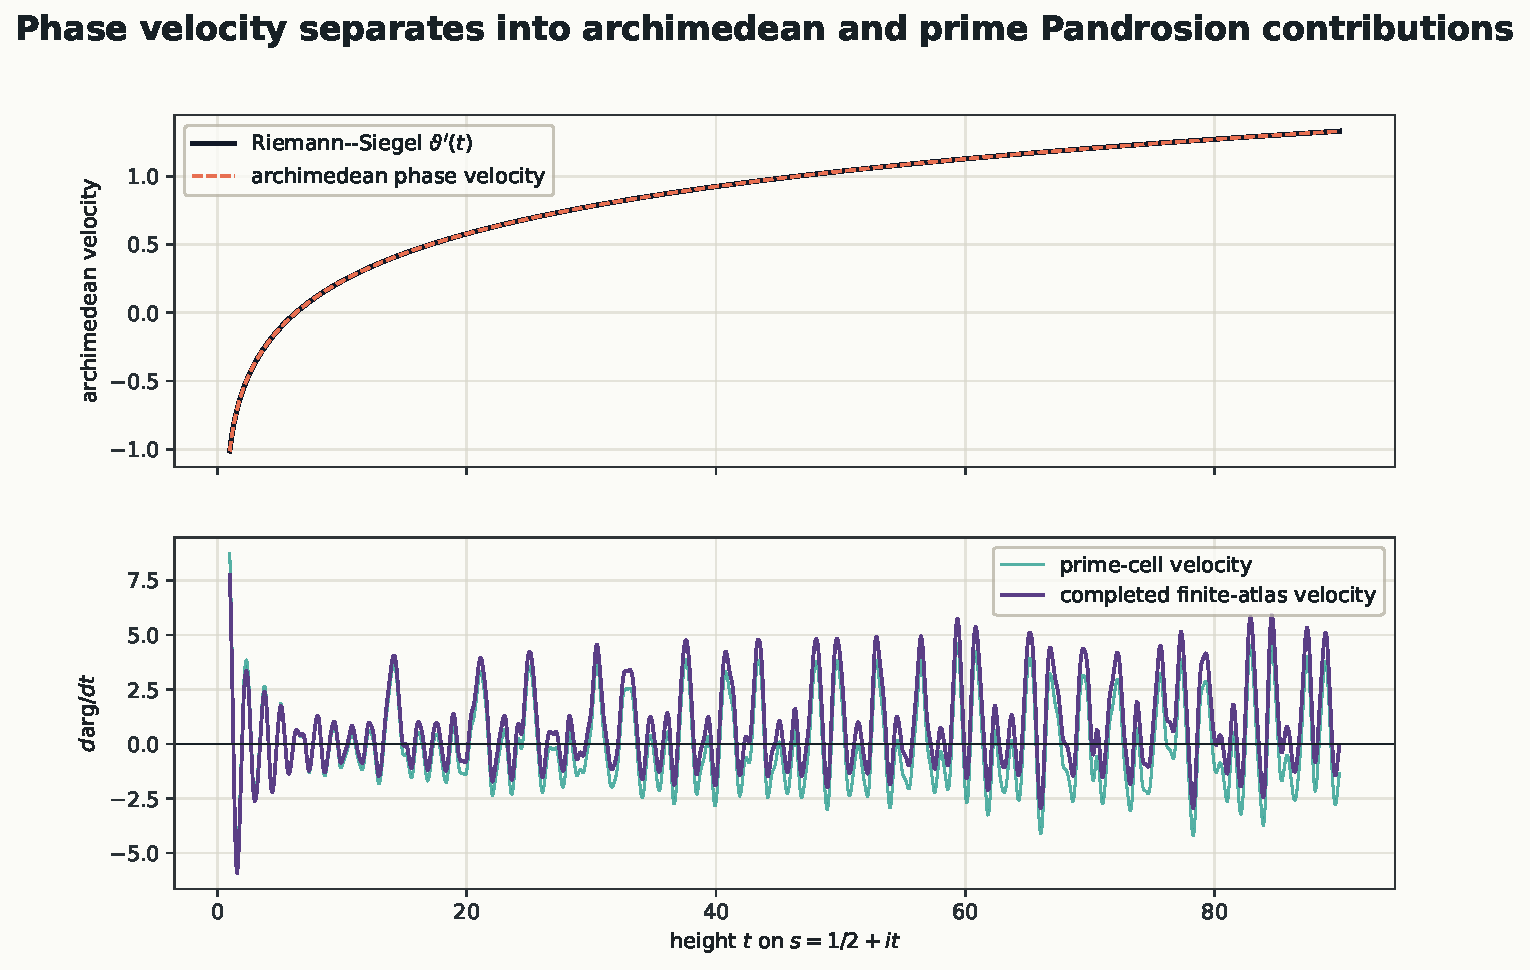
\includegraphics[width=0.96\linewidth]{026_completed_phase_velocity.pdf}
\caption{The completed phase velocity splits into an archimedean part and a
finite prime-cell part.  The upper panel verifies the Riemann--Siegel
archimedean velocity; the lower panel adds the finite Euler-Pandrosion
contribution.}
\label{fig:phase-velocity}
\end{figure}

\section{Phase destruction}

A zero cannot be detected by phase alone.  A phase condition can be satisfied
while the amplitude is large.  The completed finite atlas therefore suggests a
two-condition test:
\[
        |\X_{\Pset,N}(1/2+it)|\ \text{small},
        \qquad
        \arg\X_{\Pset,N}(1/2+it)\equiv \frac{\pi}{2}\pmod\pi
\]
or an equivalent Hardy-real normalization.

\begin{definition}[Finite phase-destruction candidate]
A height \(t\) is a finite \((\Pset,N)\)-candidate if it is a local minimum of
\(|\X_{\Pset,N}(1/2+it)|\) and the phase of \(\X_{\Pset,N}(1/2+it)\) lies
within a prescribed tolerance of a destructive phase class modulo \(\pi\).
\end{definition}

\begin{figure}[htbp]
\centering
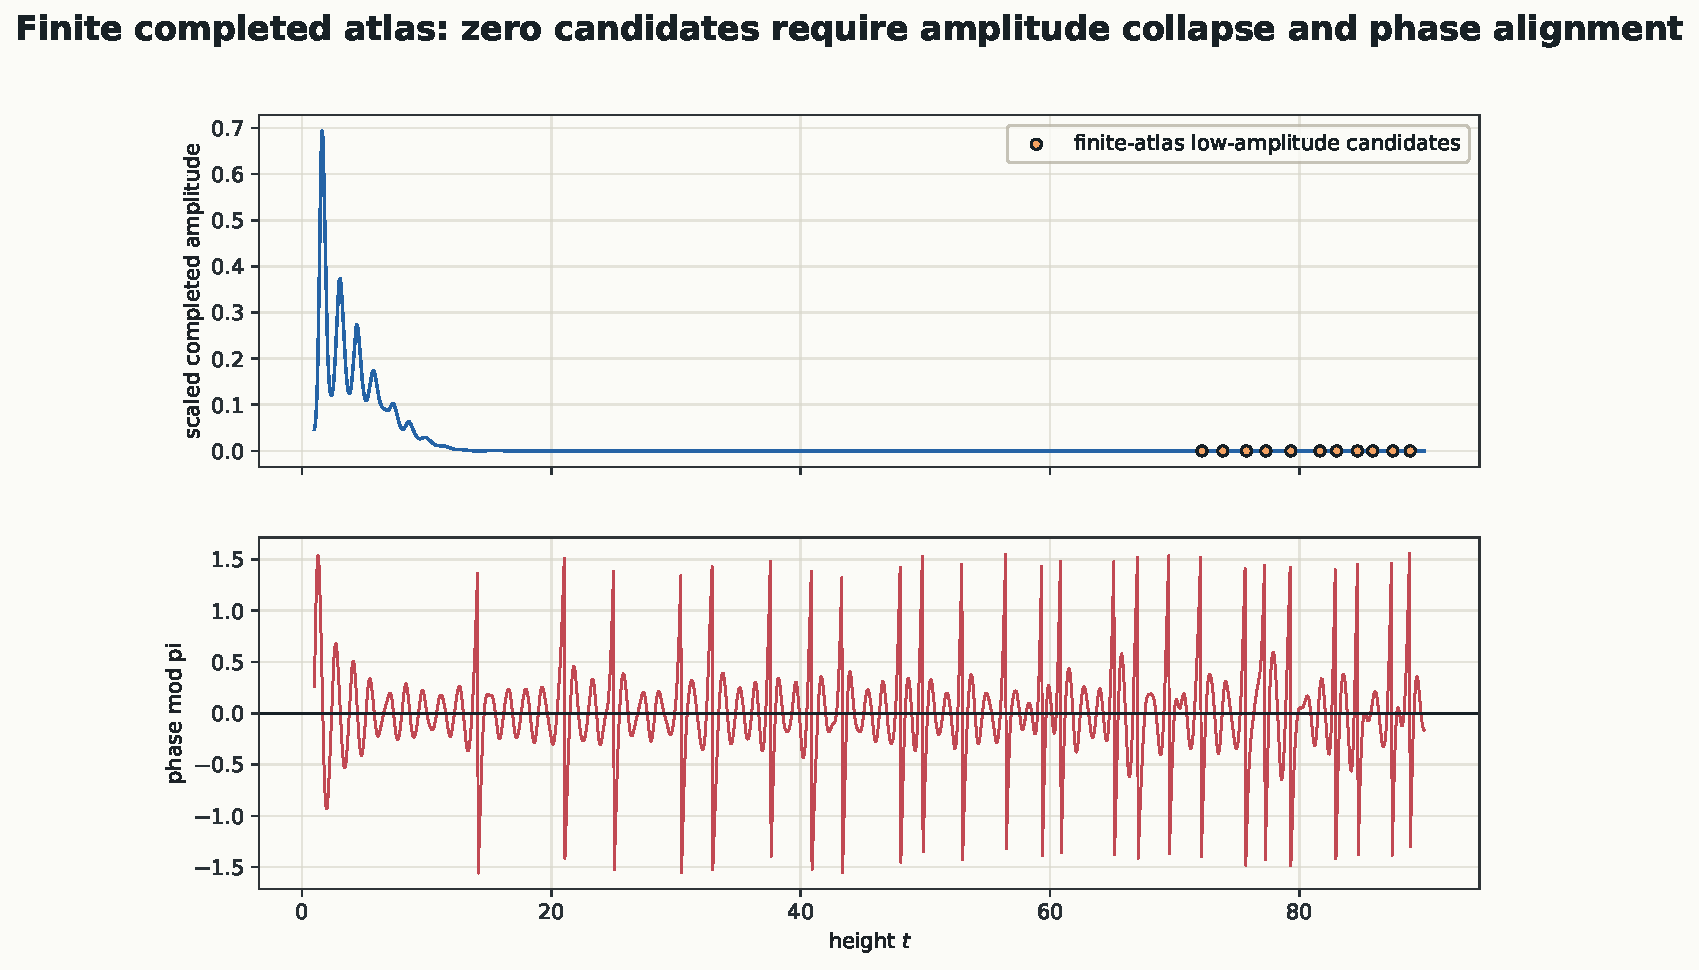
\includegraphics[width=0.96\linewidth]{026_phase_amplitude_candidates.pdf}
\caption{Finite completed atlas illustration.  These plotted candidates are
not zeta zeros; they show the intended two-filter logic: low completed
amplitude plus phase alignment.}
\label{fig:phase-amplitude}
\end{figure}

\begin{conjecture}[Completed Pandrosion phase-destruction principle]
There is a renormalized exhaustion of prime sets \(\Pset_L\), depths \(N_L\),
and archimedean normalizations such that the finite phase-destruction
candidates of \(\X_{\Pset_L,N_L}\) converge, with multiplicity, to the
nontrivial zeros of the completed zeta function \(\xi(s)\).
\end{conjecture}

\begin{remark}
This conjecture is deliberately weaker than the Riemann hypothesis.  It says
that a Pandrosion phase model can approximate the zero set of \(\xi\).  A
stronger version would assert that stable limiting candidates can occur only
on the balanced line \(\Re(s)=1/2\), using the chart imbalance from Paper 025.
\end{remark}

\section{What is new relative to 025}

Paper 025 proves the finite direct/reciprocal balance theorem:
\[
        \E_+(\sigma)=\E_\infty(\sigma)
        \quad\Longleftrightarrow\quad
        \sigma=\frac12.
\]
That explains why the critical line is geometrically selected by the
prime-atlas charts.  It does not supply the zero dynamics.

This paper adds:
\begin{enumerate}[leftmargin=2em]
\item the archimedean gamma chart \(C(s)\);
\item the completed finite atlas \(\X_{\Pset,N}\);
\item an exact phase-velocity formula;
\item the Riemann--Siegel theta derivative as the archimedean velocity;
\item a two-filter zero-candidate principle: amplitude collapse plus phase
alignment.
\end{enumerate}

\section{Research targets}

The phase calculus gives several concrete next tasks.

\begin{enumerate}[leftmargin=2em]
\item Define the correct renormalization of \(\X_{\Pset,N}\) in the critical
strip, since raw Euler products do not converge there.
\item Compare finite phase-destruction candidates with the Riemann--Siegel
zero-counting formula.
\item Prove compactness for candidate sequences under prime-set/depth
exhaustion.
\item Add the chart-imbalance energy from Paper 025 and prove that off-line
candidates are unstable under completion.
\item Relate the completed Pandrosion phase velocity to the explicit formula,
where primes and zeros already appear as dual spectral objects.
\end{enumerate}

\section{Conclusion}

The most promising Pandrosion--zeta route is not a classical finite
interpolation identity.  It is a completed atlas: prime Euler factors as
geometric Pandrosion cells, the gamma factor as the archimedean chart, and the
critical line as the direct/reciprocal balance locus.  Paper 025 supplied the
balance theorem.  This paper supplies the finite phase calculus.  The resulting
program is precise: construct a renormalized completed Pandrosion atlas whose
phase-destruction candidates converge to the zeros of \(\xi\), then use the
chart imbalance to investigate why stable candidates should be confined to the
critical line.

\begin{thebibliography}{99}

\bibitem{Besevic000}
I. Besevic, \emph{A Monomial Pandrosion Scheme: Contraction, Chart Scaling,
and Steffensen Acceleration for \(z^p=x\)}, preprint, May 2026.

\bibitem{Besevic025}
I. Besevic, \emph{Pandrosion Prime Atlases and the Riemann Critical Line},
preprint, May 2026.

\bibitem{Riemann}
B. Riemann, ``Ueber die Anzahl der Primzahlen unter einer gegebenen
Grosse,'' \emph{Monatsberichte der Berliner Akademie}, 1859.

\bibitem{Titchmarsh}
E. C. Titchmarsh, \emph{The Theory of the Riemann Zeta-Function}, 2nd ed.,
revised by D. R. Heath-Brown, Oxford University Press, 1986.

\bibitem{Edwards}
H. M. Edwards, \emph{Riemann's Zeta Function}, Dover, 2001.

\bibitem{Ivic}
A. Ivic, \emph{The Riemann Zeta-Function: Theory and Applications}, Dover,
2003.

\bibitem{RiemannSiegel}
C. L. Siegel, ``Uber Riemanns Nachlass zur analytischen Zahlentheorie,''
\emph{Quellen und Studien zur Geschichte der Mathematik, Astronomie und
Physik}, Abteilung B, 2, 45--80, 1932.

\end{thebibliography}

\end{document}
